\documentclass[aspectratio=169]{beamer}

%\usepackage[T2A]{fontenc}
\usepackage[utf8]{inputenc}
\usepackage[russian]{babel}
\usepackage{graphicx, epsfig}
\usepackage{amsmath,mathrsfs,amsfonts,amssymb}
\usepackage{floatflt}
\usepackage{epic,ecltree}
\usepackage{mathtext}
\usepackage{fancybox}
\usepackage{fancyhdr}
\usepackage{multirow}
\usepackage{enumerate}
\usepackage{epstopdf}
\usepackage{multicol}
%\usepackage{algorithm}
%\usepackage[noend]{algorithmic}
\usepackage{tikz}
\usepackage{blindtext}
\usetheme{default}%{Singapore}%{Warsaw}%{Warsaw}%{Darmstadt}
\usecolortheme{default}

% Теоремы
\newtheorem{rustheorem}{Теорема}
\newtheorem{russtatement}{Утверждение}
\newtheorem{rusdefinition}{Определение}

%\setbeamerfont{title}{size=\Huge}
\setbeamertemplate{footline}[page number]{}

\setbeamertemplate{section in toc}[sections numbered]


\makeatletter
\newcommand\HUGE{\@setfontsize\Huge{35}{40}}
\makeatother    

%\setbeamerfont{title}{size=\HUGE}
\beamertemplatenavigationsymbolsempty

% latin bold lower
\newcommand{\ba}{\mathbf{a}} 
\newcommand{\bc}{\mathbf{c}} 
\newcommand{\be}{\mathbf{e}} 
\newcommand{\bh}{\mathbf{h}} 
\newcommand{\bp}{\mathbf{p}} 
\newcommand{\bt}{\mathbf{t}} 
\newcommand{\bs}{\mathbf{s}} 
\newcommand{\bu}{\mathbf{u}} 
\newcommand{\bv}{\mathbf{v}} 
\newcommand{\bw}{\mathbf{w}} 
\newcommand{\bx}{\mathbf{x}} 
\newcommand{\by}{\mathbf{y}} 
\newcommand{\bz}{\mathbf{z}} 

% latin bold upper
\newcommand{\bA}{\mathbf{A}} 
\newcommand{\bB}{\mathbf{B}} 
\newcommand{\bC}{\mathbf{C}} 
\newcommand{\bI}{\mathbf{I}} 
\newcommand{\bJ}{\mathbf{J}} 
\newcommand{\bL}{\mathbf{L}} 
\newcommand{\bM}{\mathbf{M}} 
\newcommand{\bP}{\mathbf{P}}
\newcommand{\bQ}{\mathbf{Q}} 
\newcommand{\bR}{\mathbf{R}} 
\newcommand{\bT}{\mathbf{T}} 
\newcommand{\bU}{\mathbf{U}} 
\newcommand{\bV}{\mathbf{V}} 
\newcommand{\bW}{\mathbf{W}} 
\newcommand{\bX}{\mathbf{X}} 
\newcommand{\bY}{\mathbf{Y}} 
\newcommand{\bZ}{\mathbf{Z}} 

% latin cal upper
\newcommand{\cF}{\mathcal{F}} 
\newcommand{\cG}{\mathcal{G}} 
\newcommand{\cI}{\mathcal{I}} 
\newcommand{\cL}{\mathcal{L}} 
\newcommand{\cM}{\mathcal{M}} 
\newcommand{\cN}{\mathcal{N}} 
\newcommand{\cS}{\mathcal{S}} 
\newcommand{\cT}{\mathcal{T}} 
\newcommand{\cW}{\mathcal{W}} 
\newcommand{\cX}{\mathcal{X}} 
\newcommand{\cZ}{\mathcal{Z}} 

% latin bb upper
\newcommand{\bbE}{\mathbb{E}} 
\newcommand{\bbI}{\mathbb{I}} 
\newcommand{\bbP}{\mathbb{P}} 
\newcommand{\bbR}{\mathbb{R}}
\newcommand{\bbX}{\mathbb{X}} 
\newcommand{\bbY}{\mathbb{Y}}
\newcommand{\bbW}{\mathbb{W}} 

% greek bold lower
\newcommand{\bepsilon}{\boldsymbol{\epsilon}} 
\newcommand{\btheta}{\boldsymbol{\theta}} 
\newcommand{\blambda}{\boldsymbol{\lambda}} 
\newcommand{\bpi}{\boldsymbol{\pi}} 
\newcommand{\bmu}{\boldsymbol{\mu}} 
\newcommand{\bsigma}{\boldsymbol{\sigma}} 
\newcommand{\bphi}{\boldsymbol{\phi}} 

% greek bold upper
\newcommand{\bSigma}{\boldsymbol{\Sigma}} 

\DeclareMathOperator*{\argmin}{arg\,min}
\DeclareMathOperator*{\argmax}{arg\,max}
\newcommand{\createtitle}{\title[\hbox to 56mm{Модели распространения эпидемий, в частности, COVID-19 как модель стохастической химической кинетики\hfill\insertframenumber\,/\,\inserttotalframenumber}]
	{\vspace{1cm} \\ \LARGE{\textbf{Модели распространения эпидемий, в частности, COVID-19 как модель стохастической химической кинетики}}}
	\author[Никита Киселев]{
    Бабкин Петр Б05-003\\
    Дорин Даниил Б05-003\\
    Киселев Никита Б05-003\\
    Крейнин Матвей Б05-003\\
    Никитина Мария Б05-003
    }
	\institute[МФТИ(НИУ)]{
	Московский физико-технический институт\\
    (национальный исследовательский университет)\\
    Физтех-школа прикладной математики и информатики\\
    } 
	\date{Москва~--- 2023}
}

\usepackage{tikz}
\usetikzlibrary{arrows,shapes,positioning,shadows,trees}

\newcommand\myfootnote[1]{%
  \tikz[remember picture,overlay]
  \draw (current page.south west) +(1in + \oddsidemargin,0.5em)
  node[anchor=south west,inner sep=0pt]{\parbox{\textwidth}{%
      \rlap{\rule{10em}{0.4pt}}\raggedright\scriptsize \textit{#1}}};}

\newcommand\myfootnotewithlink[2]{%
  \tikz[remember picture,overlay]
  \draw (current page.south west) +(1in + \oddsidemargin,0.5em)
  node[anchor=south west,inner sep=0pt]{\parbox{\textwidth}{%
      \rlap{\rule{10em}{0.4pt}}\raggedright\scriptsize\href{#1}{\textit{#2}}}};}
      
\AtBeginSection[]
      {
      	\begin{frame}{Outline}
      		\tableofcontents[currentsection]
      	\end{frame}
      }
      \AtBeginSubsection[]{
      	\begin{frame}{Outline}
      		\tableofcontents[currentsection,currentsubsection]
      	\end{frame}
}
\createtitle

% import citation package
\usepackage[backend=biber, style=authoryear]{biblatex}
\addbibresource{../paper/references.bib}
\AtBeginBibliography{\small}

% footnote without number
\newcommand\blfootnote[1]{
\begingroup
\renewcommand\thefootnote{}\footnote{#1}
\addtocounter{footnote}{-1}
\endgroup
}

\usepackage{algorithm}
\usepackage[noend]{algpseudocode}

\renewcommand{\algorithmicrequire}{\textbf{Input:}}
\renewcommand{\algorithmicensure}{\textbf{Output:}}

\newcommand{\prob}[1]{\mathbb{P}\left(#1\right)}

\begin{document}

%=======
\begin{frame}[noframenumbering,plain]
	%\thispagestyle{empty}
	\titlepage
\end{frame}
%=======
\begin{frame}{Модель SIR (без рождения и смерти)}
    Пусть в популяции из $N$ человек распространяется эпидемия. Введем в рассмотрение функции
    \begin{enumerate}
        \item $S(t)$~--- число людей, еще не переболевших вирусом, но восприимчивых к заболеванию, в момент времени $t$;
        \item $I(t)$~--- число людей, инфицированных вирусом, способных заразить восприимчивых;
        \item $R(t)$~--- число людей, получивших иммунитет.
    \end{enumerate}
    В модели SIR вводятся следующие естественные предположения:
    \begin{enumerate}
        \item Суммарное число людей в популяции остается постоянным и равным $N$;
        \item Число заболеваний пропорционально числу контактов между людьми;
        \item Скорости заражения и выздоровления не меняются с течением времени.
    \end{enumerate}
    Из определения ясно, что на данные функции накладывается естественное условие:
    \[
        S(t) + I(t) + R(t) \equiv N.
    \]
\end{frame}
%=======
\begin{frame}{Модель SIR (без рождения и смерти)}
    Составим систему уравнений, которая бы на макроскопическом уровне описывала то, что происходит в популяции. Рассмотрим некоторый промежуток времени $\Delta t$. Пусть за это время произошло число заражений $\Delta I = - \Delta S$ и число выздоровлений $\Delta R$, тогда доля зараженных людей в популяции изменилась на $\Delta I / N = - \Delta S / N$, а доля выздоровевших на $\Delta R / N$. С другой стороны, заметим, что каждую из этих величин можно выразить следующим образом:
    \begin{align*}
        \frac{\Delta S}{N} &= - \dfrac{I}{N} \cdot \dfrac{S}{N} \cdot \beta \cdot \Delta t \\
        \frac{\Delta I}{N} &= \dfrac{I}{N} \cdot \dfrac{S}{N} \cdot \beta \cdot \Delta t - \dfrac{I}{N} \cdot \gamma \cdot \Delta t \\
        \frac{\Delta R}{N} &= \dfrac{I}{N} \cdot \gamma \cdot \Delta t
    \end{align*}
    Здесь $I/N$ и $S/N$~--- вероятности встретить зараженного и восприимчивого человека в популяции соответственно, $\beta$~--- скорость заражения, а $\gamma$~--- скорость выздоровления зараженного человека.
\end{frame}
%=======
\begin{frame}{Модель SIR (без рождения и смерти)}
    При промежутке времени $\Delta t \to 0$ динамика системы может быть выражена системой обыкновенных дифференциальных уравнений (СОДУ):
    \begin{align*}
        \frac{dS}{dt} &= - \beta \dfrac{IS}{N} \\
        \frac{dI}{dt} &= \beta \dfrac{IS}{N} - \gamma I \\
        \frac{dR}{dt} &= \gamma I
    \end{align*}
    Из введенной в рассмотрение системы сразу же следует, что
    \begin{equation*}
        \frac{dS}{dt} + \frac{dI}{dt} + \frac{dR}{dt} = 0,
    \end{equation*}
    откуда
    \begin{equation*}
        S(t) + I(t) + R(t) = \mathrm{const} = N.
    \end{equation*}
\end{frame}
%=======
\begin{frame}{Модель SIR (без рождения и смерти)}
    Формально мы получили СОДУ, описывающую макроскопическое состояние популяции. Проблема в том, что функции $S(t)$, $I(t)$ и $R(t)$ на самом деле являются \alert{случайными}. Т.е. в задаче рассматривается динамика некоторого случайного процесса. Но, решая систему, мы получаем \alert{детерминированные} функции! 
    \begin{block}{Идея}
        Подойти к решению задачи с точки зрения стохастической химической кинетики.
    \end{block}
\end{frame}
%=======
\begin{frame}{Модели стохастической химической кинетики}
    Задана некоторая макросистема. Пусть ее состояние характеризуется неотрицательным целочисленными вектором $n \in \mathbb{R}^m$ (по сути это просто число частиц/людей в определенном состоянии). И пусть в системе происходят случайные превращения (химические реакции).
    \begin{block}{Интенсивность реакции}
        Пусть $n \to n - \alpha + \beta, \ (\alpha, \beta) \in J$~--- все возможные типы реакций, где $\alpha$ и $\beta$~--- вектора с неотрицательными целочисленными компонентами. Введем интенсивность реакции:
        \[ \lambda_{(\alpha, \beta)}(n) = \lambda_{(\alpha, \beta)}(n \to n - \alpha + \beta) = N^{1 - \sum\limits_{i} \alpha_i} K^{\alpha}_{\beta} \prod_{i: \alpha_i > 0} n_i \cdot \ldots \cdot (n_i - \alpha_i + 1), \]
        где $K^{\alpha}_{\beta} \geqslant 0$~--- константа реакции; при этом $\sum\limits_{i=1}^m n_i(t) \equiv N \gg 1$. Другими словами, $\lambda_{(\alpha, \beta)}(n)$~--- вероятность осуществления в единицу времени перехода $n \to n - \alpha + \beta$.
    \end{block}
\end{frame}
%=======
\begin{frame}{Модели стохастической химической кинетики}
    Возникающий марковский процесс считается неразложимым (все состояния являются сообщающимися, т.е. каждое достижимо из каждого).
    \begin{rustheorem}[Куртц]
        Если существует 
        \[ \lim_{N \to \infty} \dfrac{n(0)}{N} = c(0), \]
        где $K^{\alpha}_{\beta} := K^{\alpha}_{\beta}(n/N)$, а $m$ и $J$ не зависят от $N$, то для любого $t > 0$ с вероятностью 1 существует
        \[ \lim_{N \to \infty} \dfrac{n(t)}{N} = c(t) \quad \Big[ \text{т.е. } \dfrac{n(t)}{N} \xrightarrow{\text{п.н.}} c(t) \Big], \]
        где $c(t)$~--- не случайная вектор-функция, удовлетворяющая СОДУ Гульдберга-Вааге (закон действующих масс):
        \[ \dfrac{dc_i}{dt} = \sum\limits_{(\alpha, \beta) \in J} \left( \beta_i - \alpha_i \right) K^{\alpha}_{\beta} \prod_j c_j^{\alpha_j}. \]
    \end{rustheorem}
\end{frame}
%=======
\begin{frame}{Модели стохастической химической кинетики}
    Более того, случайный процесс $n(t)/N$ слабо сходится при $N \to \infty$ к $c(t)$ на любом конечном промежутке времени. Отметим, что в каком-то смысле жизнь нелинейной динамической системы определяется линейными законами сохранения, унаследованными ею при \textcolor{blue}{каноническом скейлинге} (по сути заключающемся в замене концентраций их средними значениями).
\end{frame}
%=======
\begin{frame}{SIR как модель стохастической химической кинетики}
    Заметим, что модель SIR, изложенная в первом разделе, в действительности является моделью стохастической кинетики. В наших обозначениях 
    \[ n(t) = \begin{bmatrix} n_1(t) \\ n_2(t) \\ n_3(t) \end{bmatrix} = \begin{bmatrix} S(t) \\ I(t) \\ R(t) \end{bmatrix}, \quad n_i(t) \in \mathbb{N} \cup \{0\}, \ i = 1, 2, 3. \]
    Все возможные переходы описываются как
    \[ \mathcal{S} + \mathcal{I} \to 2 \mathcal{I}, \qquad \mathcal{I} \to \mathcal{R}. \]
    Тогда всего есть две ситуации:
    \[ \alpha^1 = \begin{bmatrix} 1 \\ 1 \\ 0 \end{bmatrix}, \quad \beta^1 = \begin{bmatrix} 0 \\ 2 \\ 0 \end{bmatrix}, \qquad \text{и} \qquad \alpha^2 = \begin{bmatrix} 0 \\ 1 \\ 0 \end{bmatrix}, \quad \beta^2 = \begin{bmatrix} 0 \\ 0 \\ 1 \end{bmatrix}. \]
\end{frame}
%=======
\begin{frame}{SIR как модель стохастической химической кинетики}
    Обозначим $\nu(t) = n(t)/N$. Тогда, предполагая, что $\nu(0) \xrightarrow{\text{п.н.}} c(0)$, имеем $\nu(t) \xrightarrow{\text{п.н.}} c(t)$, а СОДУ Гульдберга-Вааге примет вид
    \begin{align*}
        \dfrac{dc_1}{dt} &= - \beta c_1 c_2 \\
        \dfrac{dc_2}{dt} &= \beta c_1 c_2 - \gamma c_2 \\
        \dfrac{dc_3}{dt} &= \gamma c_2
    \end{align*}
    В самом деле, эта система совпадает с СОДУ, полученной в модели SIR, однако там мы не акцентировали внимание на том, что $n(t)$ вообще-то является случайным вектором и $N \gg 1$.
\end{frame}
%=======
\begin{frame}{Марковская модель распространения эпидемии}
    Попробуем получить марковскую модель описания микроскопической динамики эпидемии, которая в макромасштабе описывается моделью SIR.
    \begin{block}{Постановка задачи}
        \emph{В популяции из $N \gg 1$ человек распространяется эпидемия. Люди делятся на восприимчивых к вирусу, зараженных и переболевших. Каждый восприимчивый к вирусу человек может сопротивляться ему некоторое время, имеющее показательное распределение с параметром $\alpha(t)$, пропорциональным доле зараженных людей. Кроме того, каждый зараженный человек имеет шанс выздороветь, причем время выздоровления имеет показательное распределение с постоянным параметром $\gamma$. Известно, что в начальный момент времени $t=0$ было заражено $I_0$ человек.}
    \end{block}
\end{frame}
%=======
\begin{frame}{Марковская модель распространения эпидемии}
    Поскольку $\alpha(t) \propto I(t)/N$, то можно записать $\alpha(t) = \beta I(t)/N$, где $\beta = \mathrm{const}$.

    Аналогично введем величины $S(t)$, $I(t)$ и $R(t)$, причем $S(t) + I(t) + R(t) \equiv N$. Рассмотрим случайный процесс
    \[ \xi(t) = \begin{bmatrix} \xi_1(t) \\ \xi_2(t) \end{bmatrix} = \begin{bmatrix} S(t) \\ I(t) \end{bmatrix}, \ t \geqslant 0, \qquad \xi(0) = \begin{bmatrix} \xi_1(0) \\ \xi_2(0) \end{bmatrix} = \begin{bmatrix} S(0) \\ I(0) \end{bmatrix} = \begin{bmatrix} N - I_0 \\ I_0 \end{bmatrix}. \]
    
    Поскольку по постановке задачи приращения процесса являются независимыми, а сам процесс принимает значения из конечного множества $\{ 0, \ldots, N \} \times \{ 0, \ldots, N \}$, то мы имеем дело с непрерывной марковской цепью!
\end{frame}
%=======
\begin{frame}{Марковская модель распространения эпидемии}
    Обозначим переходные вероятности (учитывая, что цепь однородная)
    \[ p_{(s_1, i_1) \to (s_2, i_2)}(\Delta t) = \mathbb{P} \left( S(\Delta t) = s_2, I(\Delta t) = i_2 \ | \ S(0) = s_1, I(0) = i_1 \right). \]
    Распределение вероятностей состояний:
    \[ \pi_{(s, i)}(t) = \mathbb{P} \left( S(t) = s, I(t) = i \right). \]
\end{frame}
%=======
\begin{frame}{Марковская модель распространения эпидемии}
    Выведем формулы для вероятностей переходов. Рассмотрим момент времени $t \geqslant 0$ и случайную величину $\eta(t)$, равную времени до заражения случайного восприимчивого человека, начиная с момента времени $t$. Введем случайную величину $\phi(t) = \min\{ \eta_i(t) \}_{i=1}^{S(t)}$~--- время до заражения первого из $S(t)$ восприимчивых человек, начиная с момента времени $t$. Поскольку по условию задачи $\eta(t) \sim \mathrm{Exp}(\beta I(t) / N)$, то
    \[ \prob{\phi(t) < \Delta t} = 1 - \prob{\phi(t) \geqslant \Delta t} = 1 - \prod_{i=1}^{S(t)} \prob{\eta_i(t) \geqslant \Delta t} = 1 - \exp\left( - \beta \dfrac{I(t)S(t)}{N} \Delta t \right), \]
    откуда имеем, что $\phi(t) \sim \mathrm{Exp}\left( \beta I(t) S(t) / N \right)$.
    Аналогично, рассмотрев случайную величину $\psi(t)$, равную времени до выздоровления первого из $I(t)$ зараженных человек, получим, что $\psi(t) \sim \mathrm{Exp}\left( \gamma I(t) \right)$.
\end{frame}
%=======
\begin{frame}{Марковская модель распространения эпидемии}
    Теперь запишем вероятности переходов\footnotemark[1]:
    \vspace{-0.5cm}
    \begin{block}{}
        \[ \prob{\left(S(t + \Delta t), I(t + \Delta t)\right) - \left(S(t), I(t)\right) = \left(-1, 1\right)} = \]
        \[ = \prob{\phi(t) < \Delta t} \simeq \beta \dfrac{I(t)S(t)}{N} \Delta t + o(\Delta t), \]
    \end{block}
    \vspace{-1cm}
    \begin{block}{}
        \[ \prob{\left(S(t + \Delta t), I(t + \Delta t)\right) - \left(S(t), I(t)\right) = \left(0, -1\right)} = \]
        \[ = \prob{\psi(t) < \Delta t} \simeq \gamma I(t) \Delta t + o(\Delta t), \]
    \end{block}
    \vspace{-1cm}
    \begin{block}{}
        \[ \prob{\left(S(t + \Delta t), I(t + \Delta t)\right) - \left(S(t), I(t)\right) = \left(0, 0\right)} = \]
        \[ = 1 - \left(\beta \dfrac{I(t)S(t)}{N} + \gamma I(t) \right)\Delta t + o(\Delta t). \]
    \end{block}
    \footnotetext[1]{\parencite{Greenwood2009}}
\end{frame}
%=======
\begin{frame}{Марковская модель распространения эпидемии}
    Таким образом, имеем
    \begin{align*}
        p_{(s, i) \to (s+k, i+j)}(\Delta t) = 
        \begin{cases}
            \beta \dfrac{is}{N} \Delta t + o(\Delta t), & (k, j) = (-1, 1), \\
            \gamma i \Delta t + o(\Delta t), & (k, j) = (0, -1), \\
            1 - \left(\beta \dfrac{is}{N} + \gamma i \right)\Delta t + o(\Delta t), & (k, j) = (0, 0), \\
            o(\Delta t), & \text{иначе}.
        \end{cases}
    \end{align*}
\end{frame}
%=======
\begin{frame}{Марковская модель распространения эпидемии}
    Таким образом, элементы инфинитезимальной матрицы (в нашем случае~--- 4-х мерного тензора) $Q$ есть
    \begin{align*}
        q_{(s, i) \to (s+k, i+j)} = 
        \begin{cases}
            \beta \dfrac{is}{N}, & (k, j) = (-1, 1), \\
            \gamma i, & (k, j) = (0, -1), \\
            - \left(\beta \dfrac{is}{N} + \gamma i \right), & (k, j) = (0, 0), \\
            0, & \text{иначе}.
        \end{cases}
    \end{align*}
\end{frame}
%=======
\begin{frame}{Марковская модель распространения эпидемии}
    Итак, поведение цепи можно представлять себе следующим образом. В состоянии $(s, i)$ цепь находится некоторое время $t \sim \mathrm{Exp}(q_{(s, i)})$, где $q_{(s, i)} = - q_{(s, i) \to (s, i)}$. По прошествии этого времени наступает момент скачка цепи в другое состояние. В этот момент скачка цепь может попасть в произвольное состояние $(s+k, i+j)$ с вероятностью $q_{(s, i) \to (s+k, i+j)} / q_{(s, i)}$. Таким образом,
    \begin{itemize}
        \item Вероятность возникновения одного нового заражения есть
        \[ \dfrac{\left(\beta \dfrac{is}{N} \right)}{\left( \beta \dfrac{is}{N} + \gamma i \right)}, \]
        \item Вероятность одного выздоровления есть
        \[ \dfrac{\gamma i}{\left( \beta \dfrac{is}{N} + \gamma i \right)}. \]
    \end{itemize}
\end{frame}
%=======
\begin{frame}[shrink]{Марковская модель распространения эпидемии}
\begin{algorithm}[H]
\caption{Алгоритм марковской модели распространении эпидемии}\label{alg:cap}
\begin{algorithmic}[1]
\Require $\beta, \gamma, N, I_0 $
\Ensure Массивы $t$, $S$, $I$, $R$
\State Создаем массивы $t[j]$, $S[j]$, $I[j]$, $R[j]$
\State Инициализируем $j=0$, $t[j]=0$, $S[j]=0$, $I[j]=0$, $R[j]=0$
\While {$I[j] > 0$}
\State $a = \beta I[j] S[j] / N$, $b = \gamma I[j]$
\State $p_1 = a / (a + b)$ \Comment{вероятность заражения} 
\State $p_2 = b / (a + b)$ \Comment{вероятность выздоровления}
\State Сэмплируем $u_1, u_2 \sim U[0, 1]$
\State $t[j+1] = t[j] - \ln(u_1) / (a + b)$
\If{$0 < u_2 \leqslant p_1$}
\State $S[j+1] = S[j] - 1$, $I[j+1] = I[j] + 1$, $R[j+1] = R[j]$
\ElsIf{$p_1 < u_2 \leqslant p_1 + p_2$}
\State $S[j+1] = S[j]$, $I[j+1] = I[j] - 1$, $R[j+1] = R[j] + 1$
\Else
\State $S[j+1] = S[j]$, $I[j+1] = I[j]$, $R[j+1] = R[j]$
\EndIf
\EndWhile

\end{algorithmic}
\end{algorithm}

\end{frame}
%=======
\begin{frame}{Вычислительный эксперимент}
\begin{center}
    \begin{minipage}[t]{0.47\columnwidth}
        \begin{center}
            СОДУ
        \end{center}
        \vspace{-0.5cm}
		\begin{figure}
			\centering
			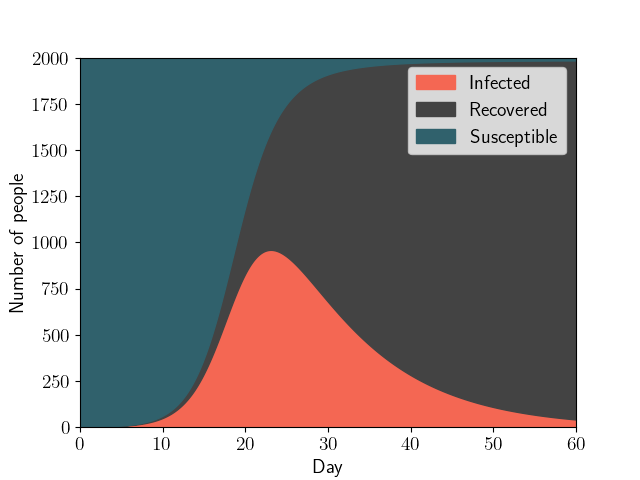
\includegraphics[width=\linewidth]{slides/SIR.png}
		\end{figure}
	\end{minipage}
	\begin{minipage}[t]{0.47\columnwidth}
        \begin{center}
            Марковская цепь
        \end{center}
        \vspace{-0.5cm}
		\begin{figure}
			\centering
			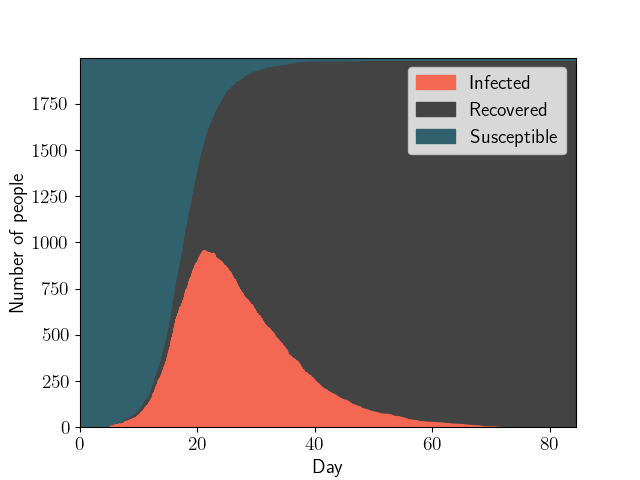
\includegraphics[width=\linewidth]{slides/stochSIR.png}
		\end{figure}
	\end{minipage}
\end{center}
\end{frame}


\begin{frame}{Вычислительный эксперимент}
\begin{center}
    \begin{minipage}[t]{0.47\columnwidth}
        \begin{center}
            СОДУ
        \end{center}
        \vspace{-0.5cm}
		\begin{figure}
			\centering
			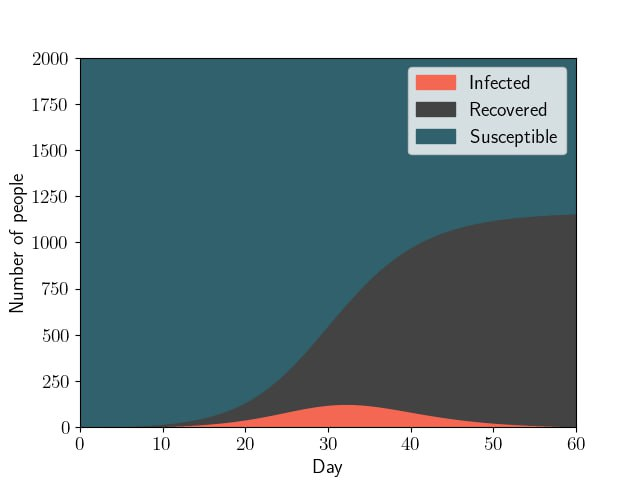
\includegraphics[width=\linewidth]{slides/SIR_2.jpeg}
		\end{figure}
	\end{minipage}
	\begin{minipage}[t]{0.47\columnwidth}
        \begin{center}
            Марковская цепь
        \end{center}
        \vspace{-0.5cm}
		\begin{figure}
			\centering
			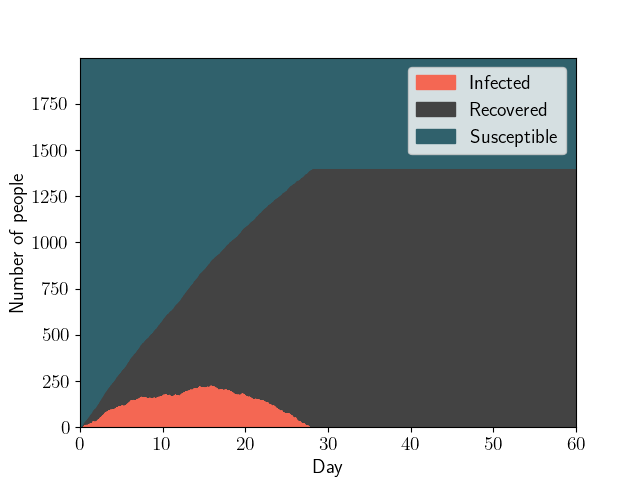
\includegraphics[width=\linewidth]{slides/stochSIR_2.png}
		\end{figure}
	\end{minipage}
\end{center}
\end{frame}

\begin{frame}{Вычислительный эксперимент}
\begin{center}
    \begin{minipage}[t]{0.47\columnwidth}
        \begin{center}
            СОДУ
        \end{center}
        \vspace{-0.5cm}
		\begin{figure}
			\centering
			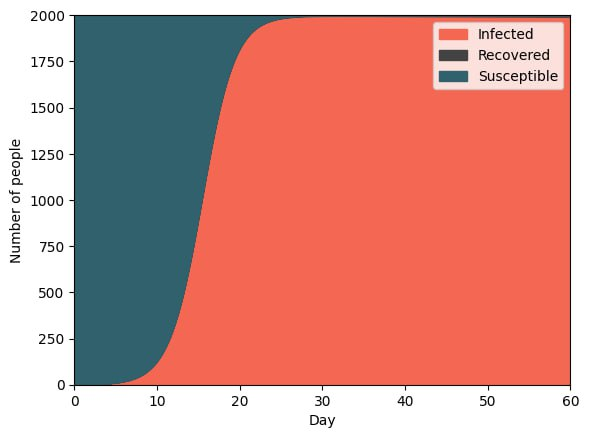
\includegraphics[width=\linewidth]{slides/SIR_3.jpeg}
		\end{figure}
	\end{minipage}
	\begin{minipage}[t]{0.47\columnwidth}
        \begin{center}
            Марковская цепь
        \end{center}
        \vspace{-0.5cm}
		\begin{figure}
			\centering
			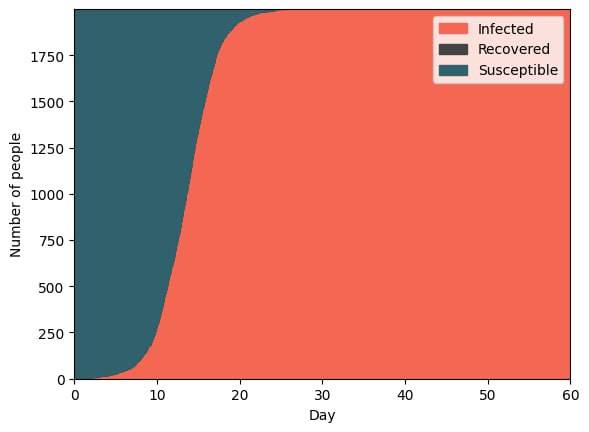
\includegraphics[width=\linewidth]{slides/stochSIR_3.jpeg}
		\end{figure}
	\end{minipage}
\end{center}
\end{frame}

\begin{frame}{Вычислительный эксперимент}
\begin{center}
    \begin{minipage}[t]{0.47\columnwidth}
        \begin{center}
            СОДУ
        \end{center}
        \vspace{-0.5cm}
		\begin{figure}
			\centering
			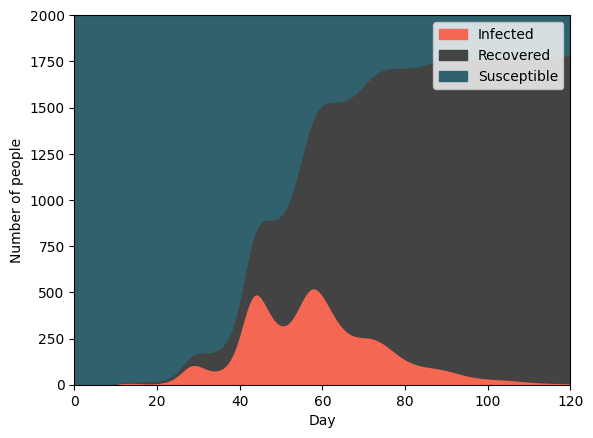
\includegraphics[width=\linewidth]{slides/sir_3waves.png}
		\end{figure}
	\end{minipage}
	\begin{minipage}[t]{0.47\columnwidth}
        \begin{center}
            Марковская цепь
        \end{center}
        \vspace{-0.5cm}
		\begin{figure}
			\centering
			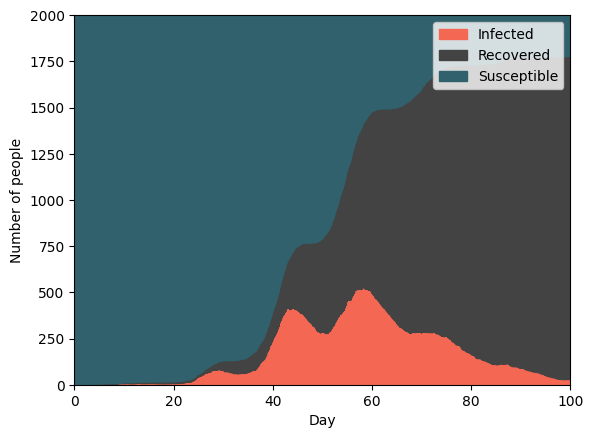
\includegraphics[width=\linewidth]{slides/stochastic_3waves.png}
		\end{figure}
	\end{minipage}
\end{center}
\end{frame}


%=======
\begin{frame}[noframenumbering]{Литература}
\nocite{*}
\printbibliography
\end{frame}
%=======

\end{document} 